\apendice{Especificación de Requisitos}

\section{Introducción}

Una muestra de cómo podría ser una tabla de casos de uso:

\section{Objetivos generales}

Este trabajo se ha realizado persiguiendo el cumplimiento de los siguientes \textbf{objetivos:}

\begin{itemize}
    \item Desarrollar un \textit{sistema software} que permita a los usuarios la corrección de ejercicios de programación.
    \item El usuario debe estar \textit{registrado} para acceder al sistema iniciando sesión.
    \item Los usuarios \textit{importarán} sus propias rúbricas en formato Markdown
    \item Los usuarios crearán sus propios prompts.
    \item La evaluación de los ejercicios se realizará mediante \textit{modelos de lenguaje LLM}.
    \item Los usuarios podrán configurar aspectos determinados del LLM usado.
    
\end{itemize}

\section{Catálogo de requisitos}
Requisitos funcionales y no funcionales para cumplir con los objetivos generales

\subsection{Requisitos funcionales}
\begin{itemize}
    \item \textbf{RF-1 - Registro de usuarios.} Los usuarios podrán registrarse mediante nombre, correo electrónico y contraseña.
    \item \textbf{RF-2 - Login de usuarios.} Los usuarios deberán iniciar sesión para usar la aplicación.
    \item \textbf{RF-3 - Importar rúbricas.} Los usuarios podrán importar sus propias rúbricas en formato Markdown.
    \begin{itemize}
        \item \textbf{RF-3.1 - Listar rúbricas.} Los usuarios podrán consultar sus rúbricas importadas.
        \item \textbf{RF-3.2 - Mostrar rubrica.} Los usuarios podrán visualizar los detalles de una rúbrica concreta.
        \item \textbf{RF-3.3 - Eliminar rúbrica.} Los usuarios podrán eliminar una rúbrica importada.
    \end{itemize}
    \item \textbf{RF-4 Crear prompts.} Los usuarios crearán sus propios prompts.
    \begin{itemize}
        \item \textbf{RF-4.1 - Listar prompts.} Los usuarios podrán consultar sus prompts creados.
        \item \textbf{RF-4.2 - Mostrar prompt.} Los usuarios podrán visualizar un prompt concreto.
        \item \textbf{RF-4.3 - Eliminar prompt.} Los usuarios podrán eliminar un prompt.
    \end{itemize}
    \item \textbf{RF-5 Configurar correcciones.} Los usuarios configurarán las correcciones.
    \begin{itemize}
        \item \textbf{RF-5.1 - Listar correcciones.} Los usuarios podrán consultar sus correcciones configuradas.
        \item \textbf{RF-5.2 - Mostrar corrección.} Los usuarios podrán visualizar un los detalles de configuración de una corrección.
        \item \textbf{RF-4.3 - Eliminar corrección.} Los usuarios podrán eliminar una corrección.
        \item \textbf{RF-5.4 - Ejecutar corrección.} Los usuarios podrán ejecutar una corrección.
    \end{itemize}
    \item \textbf{RF-6 - Configurar LLM.} Los usuarios podrán configurar aspectos determinados del LLM seleccionado.
    \begin{itemize}
        \item \textbf{RF-6.1 - Seleccionar LLM.} Los usuarios seleccionarán el LLM a usar.
        \item \textbf{RF-6.2 - Parametrizar LLM.} Los usuarios podrán modificar determinados parámetros del LLM seleccionado.
    \end{itemize}
\end{itemize}

\section{Especificación de requisitos}

Diagramas de casos de uso y detalles sobre los mismos.

\imagen{caso_de_uso_general}{Diagrama de caso de uso general}

% Caso de Uso 1 -> Registrar usuario.
\begin{table}[p]
	\centering
    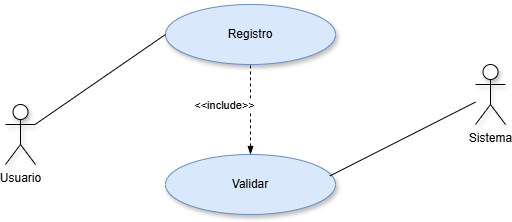
\includegraphics[width=0.7\columnwidth]{CU-1_Registro.png}
	\begin{tabularx}{\linewidth}{ p{0.21\columnwidth} p{0.71\columnwidth} }
		\toprule
		\textbf{CU-1}    & \textbf{Registro de usuario}\\
		\toprule
		\textbf{Versión}              & 1.0    \\
		\textbf{Autor}                & Pedro Antonio Abellaneda Canales \\
		\textbf{Requisitos asociados} & RF-1 \\
		\textbf{Descripción}          & Permite registrase a un usuario \\
		\textbf{Precondición}         & El usuario no puede estar logeado \\
		\textbf{Acciones}             &
		\begin{enumerate}
			\def\labelenumi{\arabic{enumi}.}
			\tightlist
			\item El usuario entra en la aplicación y accede a la página de registro
			\item El usuario introduce su email y una contraseña
            \item El usuario confirma el registro con el botón registrar
		\end{enumerate}\\
		\textbf{Postcondición}        & La aplicación redirecciona a la página de login. \\ 
                                      & Mensaje: Usuario registrado correctamente. \\
		\textbf{Excepciones}          & Mensaje \\
                                      & Mensaje \\
                                      & Mensaje \\
		\textbf{Importancia}          & Alta \\
		\bottomrule
	\end{tabularx}
	\caption{CU-1 Registrar usuario.}
\end{table}


% Caso de Uso 2 -> Login de usuario.
\begin{table}[p]
	\centering
	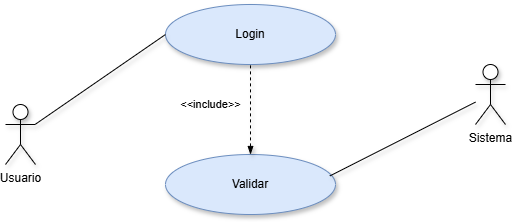
\includegraphics[width=0.7\columnwidth]{CU-2_Login.png} % Imagen encima del encabezado
	\begin{tabularx}{\linewidth}{ p{0.21\columnwidth} p{0.71\columnwidth} }
		\toprule
		\textbf{CU-2}    & \textbf{Login de usuario} \\
		\midrule
		\textbf{Versión}              & 1.0    \\
		\textbf{Autor}                & Pedro Antonio Abellaneda Canales \\
		\textbf{Requisitos asociados} & RF-2 \\
		\textbf{Descripción}          & Permite logearse a un usuario \\
		\textbf{Precondición}         & El usuario debe estar registrado \\
		\textbf{Acciones}             &
		\begin{enumerate}
			\def\labelenumi{\arabic{enumi}.}
			\tightlist
			\item El usuario entra en la aplicación y accede a la página de login.
			\item El usuario introduce su email y una contraseña.
			\item El usuario confirma pulsando el botón entrar.
		\end{enumerate} \\
		\textbf{Postcondición}        & La aplicación redirecciona a la página home. \\ 
		\textbf{Excepciones}          & Mensaje \\ 
		                              & Mensaje \\ 
		                              & Mensaje \\
		\textbf{Importancia}          & Alta \\
		\bottomrule
	\end{tabularx}
	\caption{CU-2 Login de usuario.}
	\label{tab:CU-2}
\end{table}

% Caso de Uso 3 -> Importar rúbricas
\begin{table}[p]
	\centering
	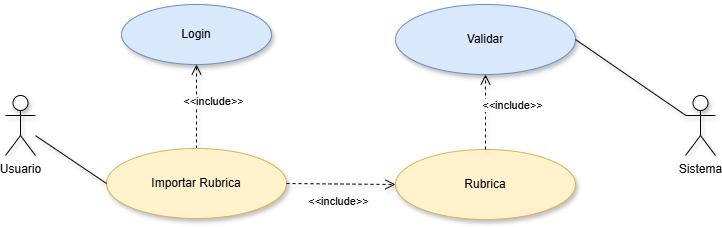
\includegraphics[width=0.9\columnwidth]{CU-3_Importar_rubrica.png} % Imagen encima del encabezado
	\begin{tabularx}{\linewidth}{ p{0.21\columnwidth} p{0.71\columnwidth} }
		\toprule
		\textbf{CU-3}    & \textbf{Importar rúbrica} \\
		\midrule
		\textbf{Versión}              & 1.0    \\
		\textbf{Autor}                & Pedro Antonio Abellaneda Canales \\
		\textbf{Requisitos asociados} & RF-3 \\
		\textbf{Descripción}          & Permite importar una rúbrica a un usuario \\
		\textbf{Precondición}         & El usuario debe estar logeado \\
		\textbf{Acciones}             &
		\begin{enumerate}
			\def\labelenumi{\arabic{enumi}.}
			\tightlist
			\item El usuario accede a la sección de rúbricas y pulsa botón nueva rúbrica.
			\item El usuario introduce un nombre para la rúbrica.
			\item El usuario importa una rúbrica.
		\end{enumerate} \\
		\textbf{Postcondición}        & La aplicación redirecciona a la página de vista de rúbricas importadas. \\ 
		\textbf{Excepciones}          & Mensaje: Error al guardar la rúbrica: Rubrica ya existente\\ 
		                              & Mensaje: El archivo subido no es un archivo Markdown \\ 
		\textbf{Importancia}          & Alta \\
		\bottomrule
	\end{tabularx}
	\caption{CU-3 Importar rúbrica.}
	\label{tab:CU-3}
\end{table}

% Caso de Uso 4 -> Listar rúbricas
\begin{table}[p]
	\centering
	%\includegraphics[width=0.9\columnwidth]{} % Imagen encima del encabezado
	\begin{tabularx}{\linewidth}{ p{0.21\columnwidth} p{0.71\columnwidth} }
		\toprule
		\textbf{CU-4}    & \textbf{Listar rúbricas} \\
		\midrule
		\textbf{Versión}              & 1.0    \\
		\textbf{Autor}                & Pedro Antonio Abellaneda Canales \\
		\textbf{Requisitos asociados} & RF-3.1 \\
		\textbf{Descripción}          & Permite ver las rúbricas del usuario \\
		\textbf{Precondición}         & El usuario debe estar logeado \\ & El usuario debe haber importado y creado alguna rúbrica \\
		\textbf{Acciones}             &
		\begin{enumerate}
			\def\labelenumi{\arabic{enumi}.}
			\tightlist
			\item El usuario accede a la sección de rúbricas

		\end{enumerate} \\
		\textbf{Postcondición}        & Se muestra la tabla con nombre y fecha de creación de cada una de las rúbricas creadas\\ 
		\textbf{Excepciones}          & \\ 
		\textbf{Importancia}          & Alta \\
		\bottomrule
	\end{tabularx}
	\caption{CU-4 Listar rúbricas.}
	\label{tab:CU-4}
\end{table}

% Caso de Uso 5 -> Mostrar rúbrica
\begin{table}[p]
	\centering
	%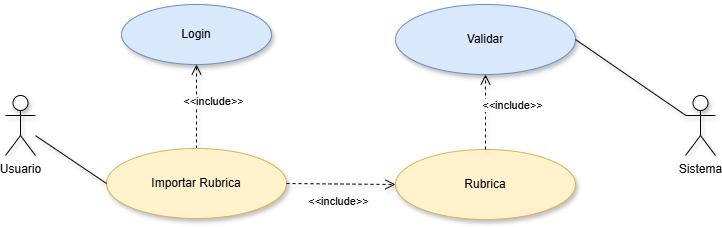
\includegraphics[width=0.9\columnwidth]{CU-3_Importar_rubrica.png} % Imagen encima del encabezado
	\begin{tabularx}{\linewidth}{ p{0.21\columnwidth} p{0.71\columnwidth} }
		\toprule
		\textbf{CU-5}    & \textbf{Mostrar rúbrica} \\
		\midrule
		\textbf{Versión}              & 1.0    \\
		\textbf{Autor}                & Pedro Antonio Abellaneda Canales \\
		\textbf{Requisitos asociados} & RF-3.2 \\
		\textbf{Descripción}          & Permite mostrar una rúbrica a un usuario \\
		\textbf{Precondición}         & El usuario debe estar logeado \\& La rúbrica debe estar creada por el usuario \\
		\textbf{Acciones}             &
		\begin{enumerate}
			\def\labelenumi{\arabic{enumi}.}
			\tightlist
			\item El usuario accede a la sección de rúbricas.
            \item El usuario busca en la tabla la rúbrica que desee.
			\item El usuario pulsa el botón mostrar.
		\end{enumerate} \\
		\textbf{Postcondición}        & La aplicación redirecciona a la página de vista de una rúbrica concreta. \\ 
		\textbf{Excepciones}          & Mensaje \\ 
		                              & Mensaje \\ 
		                              & Mensaje \\
		\textbf{Importancia}          & Alta \\
		\bottomrule
	\end{tabularx}
	\caption{CU-5 Mostrar rúbrica.}
	\label{tab:CU-5}
\end{table}

% Caso de Uso 6 -> Eliminar rúbrica
\begin{table}[p]
	\centering
	%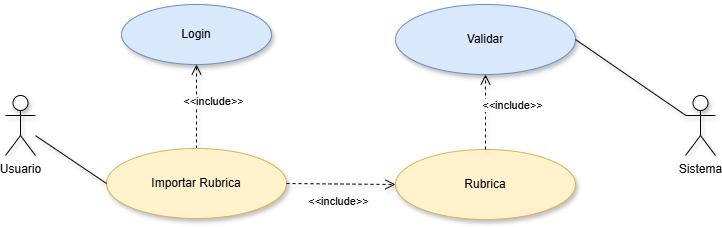
\includegraphics[width=0.9\columnwidth]{CU-3_Importar_rubrica.png} % Imagen encima del encabezado
	\begin{tabularx}{\linewidth}{ p{0.21\columnwidth} p{0.71\columnwidth} }
		\toprule
		\textbf{CU-6}    & \textbf{Eliminar rúbrica} \\
		\midrule
		\textbf{Versión}              & 1.0    \\
		\textbf{Autor}                & Pedro Antonio Abellaneda Canales \\
		\textbf{Requisitos asociados} & RF-3.3 \\
		\textbf{Descripción}          & Permite eliminar una rúbrica a un usuario \\
		\textbf{Precondición}         & El usuario debe estar logeado \\& La rúbrica debe estar creada por el usuario \\
		\textbf{Acciones}             &
		\begin{enumerate}
			\def\labelenumi{\arabic{enumi}.}
			\tightlist
			\item El usuario accede a la sección de rúbricas.
            \item El usuario busca en la tabla la rúbrica que desee.
			\item El usuario pulsa el botón eliminar.
            \item El usuario confirma la opción eliminar.
		\end{enumerate} \\
		\textbf{Postcondición}        & La aplicación redirecciona a la página rúbricas \\ 
		\textbf{Excepciones}          & Mensaje \\ 
		                              & Mensaje \\ 
		                              & Mensaje \\
		\textbf{Importancia}          & Alta \\
		\bottomrule
	\end{tabularx}
	\caption{CU-6 Eliminar rúbrica.}
	\label{tab:CU-6}
\end{table}


% Caso de Uso 7 -> Crear Prompts
\begin{table}[p]
	\centering
	%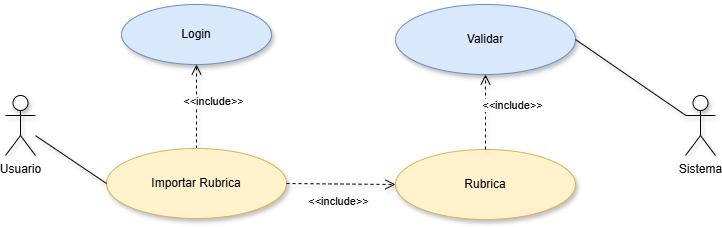
\includegraphics[width=0.9\columnwidth]{CU-3_Importar_rubrica.png} % Imagen encima del encabezado
	\begin{tabularx}{\linewidth}{ p{0.21\columnwidth} p{0.71\columnwidth} }
		\toprule
		\textbf{CU-7}    & \textbf{Crear Prompts} \\
		\midrule
		\textbf{Versión}              & 1.0    \\
		\textbf{Autor}                & Pedro Antonio Abellaneda Canales \\
		\textbf{Requisitos asociados} & RF-4 \\
		\textbf{Descripción}          & Permite crear un prompt a un usuario \\
		\textbf{Precondición}         & El usuario debe estar logeado \\
		\textbf{Acciones}             &
		\begin{enumerate}
			\def\labelenumi{\arabic{enumi}.}
			\tightlist
			\item El usuario accede a la sección de prompts y pulsa botón nuevo prompt.
            \item El usuario introduce un nombre.
			\item El usuario introduce el texto del prompt.
            \item El usuario pulsa botón importar.
		\end{enumerate} \\
		\textbf{Postcondición}        
        & 
        \begin{itemize} 
            \item La aplicación redirecciona a la página de prompts 
            \item  Mensaje: Prompt creado correctamente 
        \end{itemize}  
        \\ 
		\textbf{Excepciones}          
        & 
        \begin{itemize} 
            \item Mensaje:
            \item  Mensaje:
        \end{itemize}  
        \\ 
		\textbf{Importancia}          & Alta \\
		\bottomrule
	\end{tabularx}
	\caption{CU-7 Crear Prompts.}
	\label{tab:CU-7}
\end{table}

% Caso de Uso 8 -> Listar Prompts
\begin{table}[p]
	\centering
	%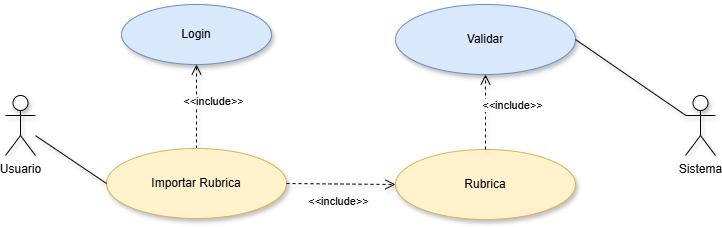
\includegraphics[width=0.9\columnwidth]{CU-3_Importar_rubrica.png} % Imagen encima del encabezado
	\begin{tabularx}{\linewidth}{ p{0.21\columnwidth} p{0.71\columnwidth} }
		\toprule
		\textbf{CU-8}    & \textbf{Listar Prompts} \\
		\midrule
		\textbf{Versión}              & 1.0    \\
		\textbf{Autor}                & Pedro Antonio Abellaneda Canales \\
		\textbf{Requisitos asociados} & RF-4.1 \\
		\textbf{Descripción}          & Permite listar los prompts de un usuario \\
		\textbf{Precondición}         
        & 
        \begin{itemize} 
            \item El usuario debe estar logeado.
            \item  El usuario debe haber creado algún prompt.
        \end{itemize}  
        \\
		\textbf{Acciones}             &
		\begin{enumerate}
			\def\labelenumi{\arabic{enumi}.}
			\tightlist
			\item El usuario accede a la sección de prompts.
		\end{enumerate} \\
		\textbf{Postcondición}        
        & 
        \begin{itemize} 
            \item Se muestra la tabla con nombre y fecha de creación de cada una de los prompts creados.
        \end{itemize}  
        \\ 
		\textbf{Excepciones}          
        & 
        \\ 
		\textbf{Importancia}          & Alta \\
		\bottomrule
	\end{tabularx}
	\caption{CU-8 Listar Prompts.}
	\label{tab:CU-8}
\end{table}